\documentclass[12pt,a4paper,UTF8]{article}
\usepackage{ctex}
\usepackage{amsmath,amscd,amsbsy,amssymb,latexsym,url,bm,amsthm}
\usepackage{epsfig,graphicx,subfigure}
\usepackage{enumitem,balance}
\usepackage{wrapfig}
\usepackage{mathrsfs,euscript}
\usepackage[usenames]{xcolor}
\usepackage{hyperref}
\usepackage[vlined,ruled,linesnumbered]{algorithm2e}
\usepackage{array}
\hypersetup{colorlinks=true,linkcolor=black}

\newtheorem{theorem}{Theorem}
\newtheorem{lemma}[theorem]{Lemma}
\newtheorem{proposition}[theorem]{Proposition}
\newtheorem{corollary}[theorem]{Corollary}
\newtheorem{exercise}{Exercise}
\newtheorem*{solution}{Solution}
\newtheorem{definition}{Definition}
\theoremstyle{definition}

\renewcommand{\thefootnote}{\fnsymbol{footnote}}

\newcommand{\postscript}[2]
 {\setlength{\epsfxsize}{#2\hsize}
  \centerline{\epsfbox{#1}}}

\renewcommand{\baselinestretch}{1.0}

\setlength{\oddsidemargin}{-0.365in}
\setlength{\evensidemargin}{-0.365in}
\setlength{\topmargin}{-0.3in}
\setlength{\headheight}{0in}
\setlength{\headsep}{0in}
\setlength{\textheight}{10.1in}
\setlength{\textwidth}{7in}
\makeatletter \renewenvironment{proof}[1][Proof] {\par\pushQED{\qed}\normalfont\topsep6\p@\@plus6\p@\relax\trivlist\item[\hskip\labelsep\bfseries#1\@addpunct{.}]\ignorespaces}{\popQED\endtrivlist\@endpefalse} \makeatother
\makeatletter
\renewenvironment{solution}[1][Solution] {\par\pushQED{\qed}\normalfont\topsep6\p@\@plus6\p@\relax\trivlist\item[\hskip\labelsep\bfseries#1\@addpunct{.}]\ignorespaces}{\popQED\endtrivlist\@endpefalse} \makeatother

\begin{document}
\noindent

%========================================================================
\noindent\framebox[\linewidth]{\shortstack[c]{
\Large{\textbf{Lab09-Network Flow}}\vspace{1mm}\\
CS214-Algorithm and Complexity, Xiaofeng Gao, Spring 2020.}}
\begin{center}
\footnotesize{\color{red}$*$ If there is any problem, please contact TA Shuodian Yu. }

\footnotesize{\color{blue}$*$ Name:Yijia Diao  \quad Student ID:518030910146 \quad Email: diao\_yijia@sjtu.edu.cn}
\end{center}
\begin{enumerate}
\item Given a weighted directed graph $G(V, E)$ and its corresponding weight matrix $W=(w_{ij})_{n \times n}$ and shortest path matrix $D=(d_{ij})_{n \times n}$, where $w_{ij}$ is the weight of edge $(v_i, v_j)$ and $d_{ij}$ is the weight of a shortest path from pairwise vertex $v_i$ to $v_j$. Now, assume the weight of a particular edge $(v_a, v_b)$ is decreased from $w_{ab}$ to $w'_{ab}$. Design an algorithm to update matrix $D$ with respect to this change, whose time complexity should be no larger than $O(n^2)$. Describe your design first and write down your algorithm in the form of pseudo-code.
    \begin{solution}
    	Since the weight of $(v_a, v_b)$ decreased, it might be in the new shortest path. So for $ \forall u,v\in V (u\ne v)$, we need to check the shortest path between them use $(v_a, v_b)$ or not. That is, compare weight($u\rightarrow v $), weight$( u\rightarrow v_a ) + w'_{ab} + $ weight$ ( v_b\rightarrow v ) $, and weight$( u\rightarrow v_b ) + w'_{ab} + $ weight$ ( v_a\rightarrow v ) $ (only if $ G $ is an undirected graph), finally save the smallest one to matrix $ D $.\\
        \begin{minipage}[t]{0.89\textwidth}
        	\begin{algorithm}[H]
        		\KwIn{Undirected Graph $G=(V,E), D=(d_{ij})_{n \times n},(v_a, v_b),w'_{ab}$.}
        		\KwOut{Updated matriax $ D $}
        		\BlankLine
        		\caption{Shortest path updating 1}
        		\label{Alg-1}
        		
        		\ForEach{$ v_i\in V $}{
        			\For{$ v_j\in V, j > i $}{
        					$ d_{ij}\leftarrow \min\{d_{ij},d_{ia}+w'_{ab} + d_{bj},d_{ib}+w'_{ab} + d_{aj}\} $\;
        					$ d_{ji}\leftarrow d_{ij}$\;
        			}
        		}
        		
        		\Return{$(d_{ij})_{n \times n}$}\;
        	\end{algorithm}
        \end{minipage}
    
    	\begin{minipage}[t]{0.89\textwidth}
    	\begin{algorithm}[H]
    		\KwIn{Directed Graph $G=(V,E), D=(d_{ij})_{n \times n},(v_a, v_b),w'_{ab}$.}
    		\KwOut{Updated matriax $ D $}
    		\BlankLine
    		\caption{Shortest path updating 2}
    		\label{Alg-2}
    		
    		\ForEach{$ v_i\in V $}{
    			\ForEach{$ v_j\in V $}{
    				\If{$ i\ne j $}{
    					$ d_{ij}\leftarrow \min\{d_{ij},d_{ia}+w'_{ab} + d_{bj}\} $\;
    				}
    			}
    		}
    		
    		\Return{$(d_{ij})_{n \times n}$}\;
    	\end{algorithm}
    \end{minipage}

    \end{solution}

	\item Given a directed graph $G$, whose vertices and edges information are introduced in data file ``SCC.in''. Please find its number of Strongly Connected Components with respect to the following subquestions.
    \begin{enumerate}
    	\item Read the code and explanations of the provided C/C++ source code ``SCC.cpp'', and try to complete this implementation.
    	\item Visualize the above selected Strongly Connected Components for this graph $G$. Use the $Gephi$ or other software you preferred to draw the graph. {\color{blue}(If you feel that the data provided in ``SCC.in'' is not beautiful, you can also generate your own data with more vertices and edges than $G$ and draw an additional graph. Notice that results of your visualization will be taken into the consideration of Best Lab.)}

    \end{enumerate}
    \begin{solution}
    	The figure is:\\
        \begin{figure}[!htbp]
        	\centering
        	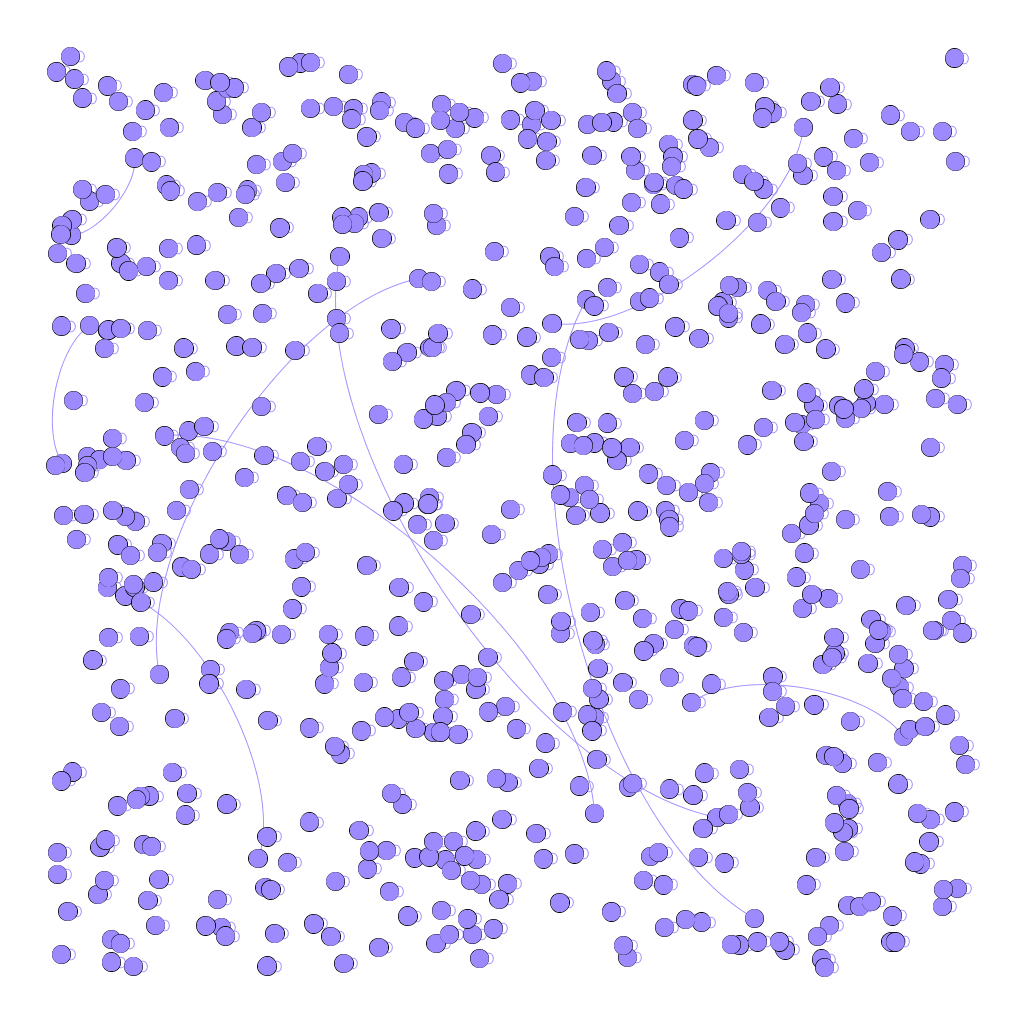
\includegraphics[width=0.5\textwidth]{Lab09-YijiaDiao.png}
        	\caption{The connection between Strongly Connected Components }
        	\label{Fig1}
        \end{figure}
    \end{solution}
	\item The \textbf{Minimum Cost Maximum Flow} problem (MCMF) is an optimization problem to find the cheapest possible way of sending the maximum amount of flow through a flow network. That is, in a flow network $G = (V, E)$ with a source $s\in V$ and a sink $t\in V$, where each edge $(u, v)\in E$ has a capacity $c(u,v) > 0$ and a cost $a(u,v) \ge 0$, find a maximum $s\text{-}t$ flow $f$ over all edges ($f(u, v) \ge 0)$, such that the total cost of $\sum_{(u, v) \in E} a(u, v) \cdot f(u, v)$ is minimized.

A common greedy approach to solve the MCMF problem can be described as follows: We can modify Ford-Fulkerson algorithm, where each time we choose the least cost path from $s$ to $t$. To do this correctly, when we add a back-edge to some edge $e$ into the residual graph, we give it a cost of $-a(e)$, representing that we get our money back if we undo the flow on it.

Note that such procedure may create a residual graph with negative-weight edges, which is not suitable for Dijkstra's Algorithm. However, motivated by Johnson's Algorithm, we can reweight the edge cost with vertex labels and convert the weight non-negative again.

Please prove the correctness of such greedy approach and implement this algorithm in C/C++. The file \emph{MCMF.in} is a test case, where the first line contains four graph parameters $n$, $m$, $s$, $t$, and the rest $m$ lines exhibit the information of $m$ edges. Each line contains four integers: $u_i$, $v_i$, $c_i$, $a_i$, denoting that there is an edge from $u_i$ to $v_i$ with capacity $c_i$ and cost $a_i$. {\color{blue}(Your source code should be named as \emph{MCMF.cpp} and output the maximum flow and minimum cost of this test case.)}

\fbox{
\begin{minipage}[t]{0.2\textwidth}
\textbf{Sample Input:}
	
	4 5 4 3 \\ 4 2 30 2 \\ 4 3 20 3 \\ 2 3 20 1 \\ 2 1 30 9 \\ 1 3 40 5
\end{minipage}
\begin{minipage}[t]{0.2\textwidth}
\textbf{Sample Output: }
	
	50 280
\end{minipage}}
\hspace{1cm}
\begin{minipage}[t]{0.45\textwidth}
\textbf{Remark:} The source code \emph{SCC.cpp}, and the input data \emph{SCC.in} and \emph{MCMF.in} are attached on the course webpage. Please include your .pdf, .tex, .cpp files for uploading with standard file names.
\end{minipage}
    \begin{proof}
        According to Ford-Fulkerson algorithm, whatever path we choose in this algorithm, we get the same overflow out of the same cut. Suppose we did not choose the shortest path to get the maximum overflow, finally the edges with a higher weight will share higher flow, while the edges with a lower weight will share lower flow. Since the sum of overflow of a special cut is a constant, higher $ a(u, v) \times$ higher $ f(u.v) $ make the cost higher than the other. 
        So we can make the conclusion that such greedy approach is correct.
    \end{proof}

\end{enumerate}






%========================================================================
\end{document}
